\documentclass[a4paper]{article}

\usepackage[spanish]{babel}
\usepackage[utf8]{inputenc}
\usepackage{amsmath}
\usepackage{graphicx}
\usepackage[colorinlistoftodos]{todonotes}
\usepackage{multicol}
\usepackage{makeidx}
\usepackage{hyperref}
\usepackage{caption}
\usepackage{amsfonts}
\usepackage{amssymb}
\usepackage{amsmath}
\usepackage[utf8]{inputenc}
\usepackage{verbatim}
\usepackage{listings}
\usepackage{algpseudocode}
\usepackage{courier}
\usepackage{enumitem}
\usepackage{placeins}



\newcommand{\BigO}[1]{\ensuremath{\operatorname{O}\bigl(#1\bigr)}}
\lstset{language=C++, showstringspaces=false, tabsize=2, breaklines=true, title=\lstname}

\usepackage{booktabs}
\usepackage[margin=1in]{geometry}

\title{Trabajo Práctico I de Teoría de las Comunicaciones}

\author{, Nicolás Lasso, , }

\date{\today}

\makeindex

\begin{document}
\newgeometry{margin=2cm}
\pagenumbering{gobble}
\raggedleft

\includegraphics[width=8cm]{caratula/logo1.jpg}\\

\raggedright
\vspace{3cm}
{\Huge \bfseries Trabajo Práctico 2}
\rule{\textwidth}{0.02in}
\large Miércoles 17 de junio de 2015 \hfill Teoría de las Comunicaciones
\vspace{1.5cm}

\normalsize
\begin{tabular}{|l@{\hspace{5ex}}c@{\hspace{5ex}}l|}
        \hline
        \rule{0pt}{1.2em}Integrante & LU & Correo electrónico\\[0.2em]
        \hline
        \rule{0pt}{1.2em} Nahuel Lascano  & 476/11 &\tt laski.nahuel@gmail.com\\[0.2em]
		\rule{0pt}{1.2em} Nicolás Lasso & 763/10 &\tt lasso.nico@gmail.com\\[0.2em]
        \rule{0pt}{1.2em} Roberto Rama  & 490/11 &\tt bertoski@gmail.com\\[0.2em]
        \rule{0pt}{1.2em} Pablo Somodi  & 818/10 &\tt psomodi@dc.uba.ar\\[0.2em]
        \hline
\end{tabular}

\vspace{1.0cm}
\raggedright

\begin{multicols}{2}

\includegraphics[width=8cm]{caratula/logo-uba.png}

\columnbreak
\vspace*{4.5cm}
\raggedleft
\textbf{Facultad de Ciencias Exactas y Naturales}\\
Universidad de Buenos Aires\\
\small
Ciudad Universitaria - (Pabellon I/Planta Baja)\\
Intendente G\"uiraldes 2160 - C1428EGA\\
Ciudad Autonoma de Buenos Aires - Rep. Argentina\\
Tel/Fax: (54 11) 4576-3359\\
http://www.fcen.uba.ar
\end{multicols}

\restoregeometry

\clearpage

\pagenumbering{arabic}

\tableofcontents

\vspace{3cm}

\clearpage

\setlength{\parindent}{10pt}

\section{Introducción}
En el presente trabajo práctico tuvimos como desafío implementar una herramienta muy común de diagnóstico de red, el traceroute.

Por medio de la misma los administradores de red pueden analizar la ruta que sigue un paquete hasta un destino dado.

Los fundamentos de dicha herramienta son muy sencillos.
Se utilizan paquetes IP para recorrer la ruta aumentando de un salto a la vez.
Esto se hace por medio del campo TTL (\textit{Time to live}) que nos permite configurar la cantidad máxima de ``saltos'' que se le permiten al paquete para llegar a destino.
Cuando un router recibe un paquete para redireccionarlo, previo a esto decrementa en 1 su TTL, si el mismo resulta igual a 0 entonces devuelve el mensaje \textbf{ICMP Time Exceeded} a la dirección de origen.

La herramienta se basa en este comportamiento para obtener la información de la ruta. La misma envía varios paquetes incrementando el TTL progresivamente desde 1 hasta que el paquete efectivamente llega a destino, y va registrando los paquetes de respuesta \textbf{ICMP Time Exceeded} que recibe de cada router.

Esta herramienta se puede implementar con paquetes ICMP, TCP o UDP, según necesidad. La herramienta default que se ofrece en cualquier distribución de Linux permite realizar el procedimiento con los tres tipos de paquetes.

\clearpage

\section{Implementación}
Los fundamentos del $traceroute$ son muy sencillos. Se utilizan paquetes IP para recorrer la ruta aumentando de un salto a la vez. Esto se hace por medio del campo TTL (\textit{Time to live}) que nos permite configurar la cantidad máxima de ``saltos'' que se le permiten al paquete para llegar a destino. Cuando un router recibe un paquete para redireccionarlo, previo a esto decrementa en 1 su TTL, si el mismo resulta igual a 0 entonces devuelve el mensaje \textbf{ICMP Time Exceeded} a la dirección de origen. La herramienta se basa en este comportamiento para obtener la información de la ruta. La misma envía varios paquetes incrementando el TTL progresivamente desde 1 hasta que el paquete efectivamente llega a destino, y va registrando los paquetes de respuesta \textbf{ICMP Time Exceeded} que recibe de cada router.

Esta herramienta se puede implementar con paquetes ICMP, TCP o UDP, según necesidad. La herramienta default que se ofrece en cualquier distribución de Linux permite realizar el procedimiento con los tres tipos de paquetes. Para implementar la herramienta utilizamos paquetes de tipo ICMP. Primeramente decidimos resolver el registro DNS a su IP correspondiente para evitar considerar el tiempo que pudiera tardar este procedimiento. Además, esto nos permite evitar el posible cambio de rutas producto de alguna universidad usando Round-robin DNS\footnote{https://en.wikipedia.org/wiki/Round-robin\_DNS}.

En el comienzo de nuestra implementación nuestra herramienta explora la ruta completa para estudiar los hosts que pertenecen a la misma. Decidimos limitar el crecimiento del $time to live$ a 35 ya que es un poco mayor que la que utilizan las herramientas provistas por Linux. De todos modos esto no afectó ya que llegamos a todos los hosts elegidos en menos saltos.

Luego de esto utilizamos la ruta descubierta para realizar 50 repeticiones de mediciones de RTT de forma incremental en el TTL. Utilizamos el promedio de las mismas con el fin de tener valores más estables. Luego de calculado este promedio realizamos las restas uno a uno entre hops sucesivos para obtener los tiempos diferenciales a partir de los acumulados.

Para normalizar los datos para el análisis calculamos el valor Z del RTT de cada hop\footnote{Recordar que nos estamos refiriendo a la diferencia entre el RTT absoluto de un hop y el anterior}, que nos da una idea de cuánto se aleja cada RTT de la media, medido en desvíos standard. Para ello usamos la ecuación facilitada por el enunciado: $$ ZRTT_i = \dfrac{RTT_i-\overline{RTT}}{SRTT}$$ donde $\overline{RTT}$ es el promedio y $SRTT$ el desvío standard de la distribución de los RTTs para una ruta dada. Esto nos permite analizar los saltos con una información estadísticamente más sólida que la diferencia absoluta medida en $ms$.

Para simular el throughput utilizamos la ecuación de Mathis
$$\frac{MSS}{EstimatedRTT * \frac{1}{1 - \sqrt{EstimatedPacketLossProbability}}}$$
donde $EstimatedRTT$ se obtiene iterando sucesivas veces la ecuación
$$\alpha * EstimatedRTT + (1 - \alpha) * SampleRTT$$
y $EstimatedPacketLossProbability$ se calcula como $$1 - \frac{\#Echo reply}{\#Echo request}$$

%TODO: Laski -- Por que se llama Estimated Packet Loss Probability si estima la probabilidad de que un paquete llegue bien? (Echos contestados sobre Echos enviados)
% Buena pregunta. Yo copié lo que decía el enunciado. Ahí lo arreglé.

Para resolver la geolocalización inicialmente decidimos incorporar una parte de código que obtuviera la información para cada IP. Esto nos trajo problemas ya que la diferencia entre los RTT no coincidía con la geolocalización real del salto. La herramienta que nos permitió encontrar estas inconsistencias fue IPLocation\footnote{http://www.iplocation.net/}, un meta-buscador que realizaba consultas a la base de IP2Location\footnote{http://www.ip2location.com/} actualizada el 01/06/2015. 
\clearpage

\section{Experimentación}
Para normalizar los datos para el análisis calculamos el valor Z del RTT de cada hop\footnote{Recordar que nos estamos refiriendo a la diferencia entre el RTT absoluto de un hop y el anterior}, que nos da una idea de cuánto se aleja cada RTT de la media, medido en desvíos standard. Para ello usamos la ecuación facilitada por el enunciado: $$ ZRTT_i = \dfrac{RTT_i-\overline{RTT}}{SRTT}$$ donde $\overline{RTT}$ es el promedio y $SRTT$ el desvío standard de la distribución de los RTTs para una ruta dada.

Esto nos permite analizar los saltos con una información estadísticamente más sólida que la diferencia absoluta medida en $ms$.

Durante la experimentación hubieron ciertas anomalías detectadas al correr los experimentos. Las mismas fueron:

\begin{itemize}
    \item Hops que no respondían. En base a este problema se generó la hipótesis de que había hops en los cuales los paquetes ICMP enviados llegaban con un \textit{Time-Exceeded} a un router que estaba configurado para no responder a estos paquetes o para filtrarlos directamente. En base a esto se configuró el método \textit{SR1()} de Scapy pa ra que dado cierto \textit{Timeout} el mismo dejara de esperar a que el router le respondiera permitiéndonos aumentar el TTL y llegar al siguiente Hop.
    \item Corridas en las cuales no se llegaba a ningún destino haciendo que el script nunca terminara incluso aumentando el TTL y el tiempo de Timeout. Con la misma Hipótesis que la anterior, realizando experimentaciones a diferentes universidades, hubieron algunas, como las que se muestran a continuación, cuyo servidor estaba configurado para no responder. Por ejemplo:
    \begin{itemize}
        \item Universidad de Tokio
        \item Melbourne University
        \item University of Mumbay
    \end{itemize}
    En este caso, lo que se realizó para constatar este comportamiento previamente fue hacer un \textit{PING()} a los destinos para corroborar si los mismos responden. De esta manera se supo si había muchos hops que no respondían, como sucedía anteriormente, entre la IP de origen y la de destino o si era efectivamente el destino.
    \item Las rutas al mismo destino cambiaban. Al correr muchas veces a la misma IP de destino, nos dimos cuenta que las rutas podían varias con lo cual no era lo suficientemente fiable el cálculo del RTT. Dado esto, cuando se detectaba que una ruta no era igual a la primer ruta obtenida, esta era descartaba y se repetía el llamado al mismo hop con el mismo TTL hasta que se obtenía una respuesta de la primer IP con dicho TTL. De esta forma se aseguró la misma ruta en todos los casos.
    \item RTTs no lineales, es decir, si bien se supone que a medida que se realizan saltos a hops más lejanos el RTT debería aumentar, esto no siempre sucedía. Al realizar las experimentaciones se notó que para cierto rango de IPs, que pertenecen a la misma región, la diferencia entre los RTT era muy grande. Por ejemplo, para dos IPs en la misma región, la primera con TTL menor, tenía un RTT mayor que la del hop siguiente que tiene un TTL mayor y un RTT significativamente menor. Otro caso que se notó fue para países muy distantes, que se suponen con un enlace submarino y una diferencia en RTTs grande, que tenían una diferencia muy pequeña. Para estos casos, tras revisar las locaciones de las IPs con el uso del sitio web: http://iplocation.net, llegamos a la conclusión de que, si bien hay rangos IPs que pertenecen a la misma región y que deberían estar relativamente cercanos, sucede que la IP física se encuentra realmente en otra locación provocando que se produzca más de un salto transatlántico y que los valores de RTT varíen de esta manera. Estos casos se pueden apreciar en la sección de resultados.  
\end{itemize}

Las universidades a las que finalmente se les realizó el tracerout fueron:

\begin{itemize}
	\item Universidad de Berkeley, California, EEUU. Con la dirección: berkley.edu
	\item Perm State University, Rusia. Con la dirección: en.psu.ru
	\item Iceland University, Iceland. Con la dirección: english.hi.is
	\item Cochin University of Scienc and Technology, Cochin, India. Con la dirección: cusat.ac.in
	\item University of Pretoria, Pretoria, South Africa. Con la dirección: up.ac.za 
\end{itemize}

Dichas universidades respondieron a los PING previos para realizar la experimentación y todas pertenecen a distintos continentes. Los resultados fueron muy variados. En varias ocaciones hay mas de un salto transatlántico los cuales fueron detectados por los RTT y serán explicados en la sección de resultados.
\clearpage

\section{Resultados}
Presentamos aquí los resultados obtenidos para cada ruta.
Para cada ruta elegida presentamos una tabla con los resultados crudos, un gráfico con puntos representando cada salto y un mapa que marca la ruta geográfica que traza la conexión establecida.

En las tablas, notar que incluímos el valor promedio del RTT absoluto de la computadora local hasta cada salto, pero como ya fue mencionado calculamos el ZRTT usando la diferencia de RTT entre un salto y el siguiente.

Para los gráficos usamos el Teorema Central del Límite, dado que tomamos suficientes muestras y las mismas son independientes, y la cuenta que efectuamos en el cálculo de ZRTT normaliza los datos. En consecuencia, los mismos pueden ser interpretados como provenientes de una distribucion normal, por lo que decidimos representarlos por encima de la campana de Gauss. Como resultado se puede observar de forma sencilla aquellos saltos que son estadisticamente significativos.

\subsection{Resultados generales}
 En todas nuestras pruebas en valor de $MSS$ obtenido fue de 1452, pero lo calculamos programáticamente antes de cada test para asegurarnos de usar el real en cada sistema utilizado.

 En todos los casos la cantidad de paquetes perdidos fue muy baja (máximo 2 de 50) por lo que no se incluye el valor de $EstimatedPacketLossProbability$ en los resultados específicos de cada ruta.

\subsection{Berkeley, EEUU}

\begin{tabular}{|c@{\hspace{5ex}}c@{\hspace{5ex}}c@{\hspace{5ex}}c@{\hspace{5ex}}c|}
 \hline
 \rule{0pt}{1.2em}IP & ZRTT & AVG\_RTT & PAIS & CIUDAD\\[0.2em]
 \hline

\rule{0pt}{1.2em} 192.168.2.1  &  0.65 & 35.35 & (Private Address) & (Private Address) \\[0.2em]
\rule{0pt}{1.2em} 200.89.164.137  &  -0.11 & 46.40 & ARGENTINA & Buenos Aires \\[0.2em]
\rule{0pt}{1.2em} 200.89.165.130  &  -0.41 & 43.80 & ARGENTINA & Buenos Aires \\[0.2em]
\rule{0pt}{1.2em} 200.89.165.222  &  -0.27 & 47.29 & ARGENTINA & Buenos Aires \\[0.2em]
\rule{0pt}{1.2em} 208.178.195.205  &  -0.43 & 43.57 & ARGENTINA & Buenos Aires \\[0.2em]
\rule{0pt}{1.2em} 67.17.68.234  &  2.86 & 191.77 & UNITED STATES & Miami \\[0.2em]
\rule{0pt}{1.2em} 4.68.111.121  &  -1.44 & 141.79 & UNITED STATES & Miami \\[0.2em]
\rule{0pt}{1.2em} 4.35.156.66  &  1.07 & 207.65 & UNITED STATES & Los Angeles \\[0.2em]
\rule{0pt}{1.2em} 137.164.11.1  &  -0.2 0& 214.70 & UNITED STATES & Cypress \\[0.2em]
\rule{0pt}{1.2em} 137.164.46.144  &  -0.31 & 216.72 & UNITED STATES & Cypress \\[0.2em]
\rule{0pt}{1.2em} 137.164.50.31  &  -0.34 & 217.22 & UNITED STATES & Cypress \\[0.2em]
\rule{0pt}{1.2em} 128.32.0.37  &  -0.28 & 220.53 & UNITED STATES & Berkeley, CA \\[0.2em]
\rule{0pt}{1.2em} 128.32.0.101  &  -0.46 & 215.66 & UNITED STATES & Berkeley, CA \\[0.2em]
\rule{0pt}{1.2em} 169.229.216.200  &  -0.31 & 217.43 & UNITED STATES & Berkeley, CA \\[0.2em]
\hline
 \end{tabular}

Podemos observar el fenómeno ya mencionado sobre RTTs menores en saltos posteriores.

Efectivamente el salto más grande (de Argentina a EEUU) se corresponde con una diferencia de RTTs sustancial, y esto se ve reflejado en el valor del ZRTT que muestra que se aleja casi tres desvíos standard de la media.

 El valor del throughput estimado para esta ruta fue de 3,864, lo cual por ahora no nos dice mucho pero será relevante al compararlo con las demás rutas.

 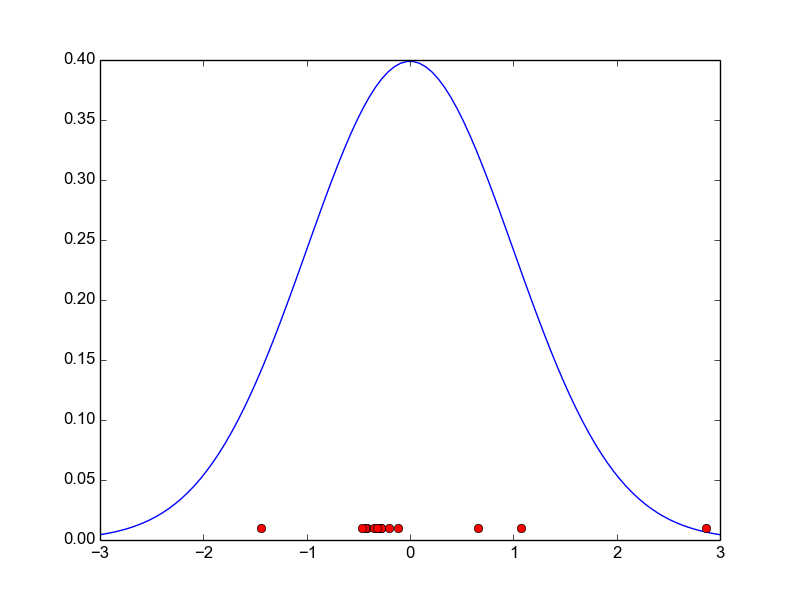
\includegraphics[width=5in]{imgs/berkeley_dist.png}
 \includegraphics[width=5in]{imgs/maps/berkeley.png}


\subsection{Cochin, India}

\begin{tabular}{|c@{\hspace{5ex}}c@{\hspace{5ex}}c@{\hspace{5ex}}c@{\hspace{5ex}}c|}
 \hline
 \rule{0pt}{1.2em}IP & ZRTT & AVG\_RTT & PAIS & CIUDAD\\[0.2em]
 \hline

\rule{0pt}{1.2em} 192.168.2.1  &  -0.01 & 35.71 & (Private Address) & (Private Address) \\[0.2em]
\rule{0pt}{1.2em} 200.89.164.181  &  -0.33 & 45.44 & ARGENTINA & Buenos Aires \\[0.2em]
\rule{0pt}{1.2em} 200.89.165.150  &  -0.43 & 43.95 & ARGENTINA & Buenos Aires \\[0.2em]
\rule{0pt}{1.2em} 195.22.220.152  &  -0.42 & 44.05 & ARGENTINA & Buenos Aires \\[0.2em]
\rule{0pt}{1.2em} 195.22.216.142  &  1.12 & 213.52 & UNITED STATES & New Orleans \\[0.2em]
\rule{0pt}{1.2em} 195.22.216.142  &  -0.43 & 212.45 & UNITED STATES & New Orleans \\[0.2em]
\rule{0pt}{1.2em} 195.22.195.102  &  1.59 & 434.06 & ITALY & Milano \\[0.2em]
\rule{0pt}{1.2em} 218.248.235.161  &  -1.76 & 286.69 & INDIA & Bangalore \\[0.2em]
\rule{0pt}{1.2em} 210.212.233.50  &  1.10 & 454.65 & INDIA & Cochin \\[0.2em]
\rule{0pt}{1.2em} 210.212.233.50  &  -0.41 & 455.32 & INDIA & Cochin \\[0.2em]
\hline
 \end{tabular}

 En una primera instancia, notamos que el IP 195.22.220.152 fue marcado como Italiano pero su RTT era demasiado bajo. Verificando contra otras bases de localizacion de IP, comprobamos que efectivamente el nodo se encuentra en Argentina, si bien su rango pertenece a Italia, ya que el ISP dueño es una corporacion Italiana.

 Nuevamente vemos una correspondencia entre el salto más largo, trasatlántico esta vez, y la diferencia entre RTTs, reflejada a su vez por el valor de ZRTT. Sin embargo también vemos una diferencia similar entre dos puntos supuestamente cercanos, y una diferencia negativa entre dos puntos supuestamente alejados.

 El valor del throughput estimado para esta ruta fue de 3,203. Comparándolo con el anterior, que el valor absoluto de RTT de la ruta sea mucho mayor afecta directamente al throughput obtenido.

 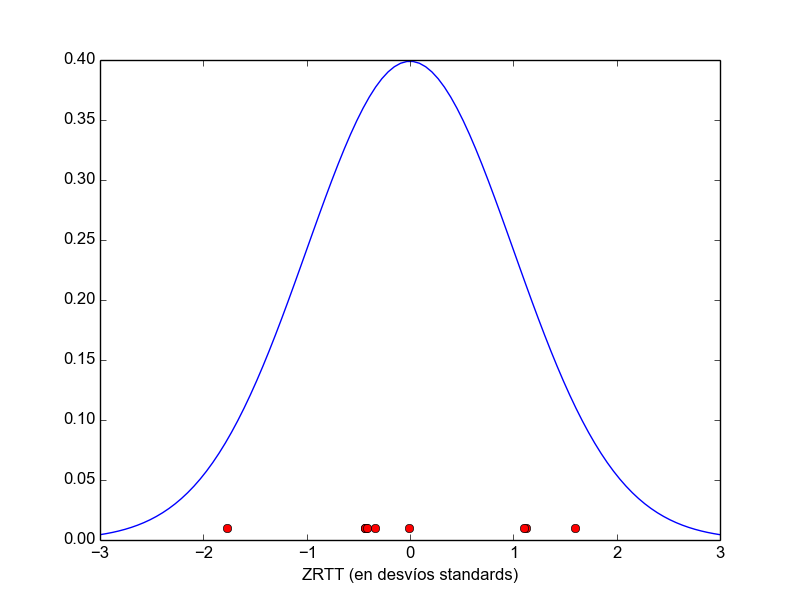
\includegraphics[width=5in]{imgs/cusat_dist.png}
 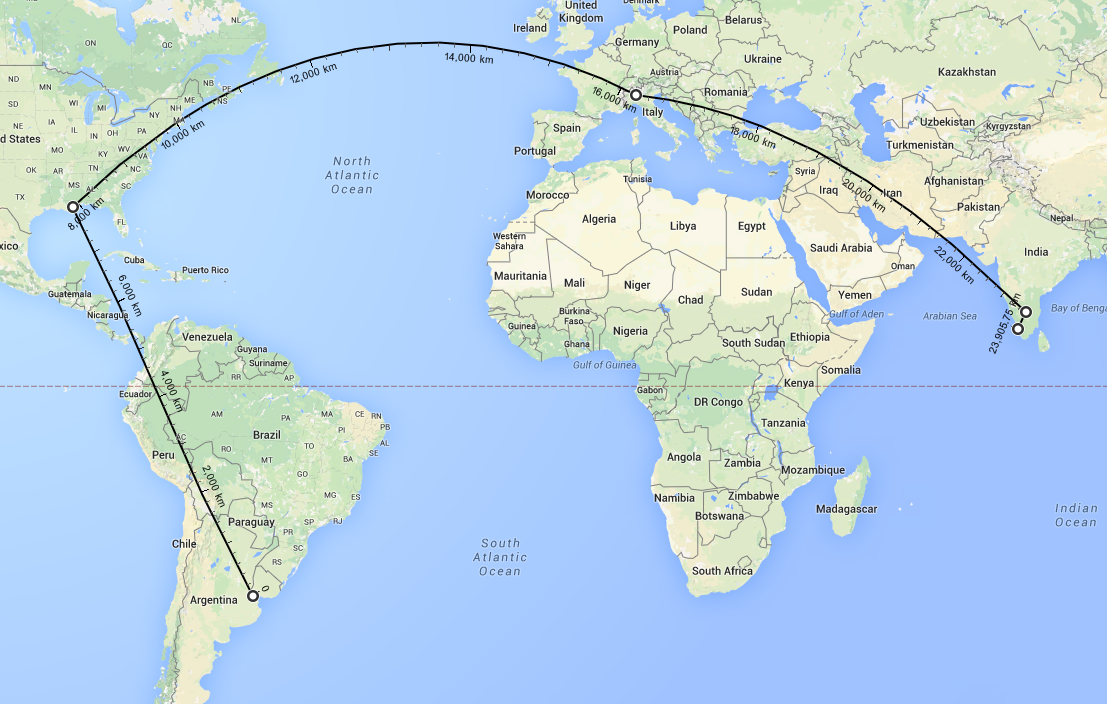
\includegraphics[width=5in]{imgs/maps/cusat.png}

\subsection{Reykjavik, Iceland}

\begin{tabular}{|c@{\hspace{5ex}}c@{\hspace{5ex}}c@{\hspace{5ex}}c@{\hspace{5ex}}c|}
 \hline
 \rule{0pt}{1.2em}IP & ZRTT & AVG\_RTT & PAIS & CIUDAD\\[0.2em]
 \hline

\rule{0pt}{1.2em} 192.168.2.1  &  0.53 & 37.3 & (Private Address) & (Private Address) \\[0.2em]
\rule{0pt}{1.2em} 200.89.164.153  &  -0.24 & 45.36 & ARGENTINA & Buenos Aires \\[0.2em]
\rule{0pt}{1.2em} 200.89.165.130  &  -0.42 & 44.90 & ARGENTINA & Buenos Aires \\[0.2em]
\rule{0pt}{1.2em} 200.89.165.222  &  -0.36 & 47.18 & ARGENTINA & Buenos Aires \\[0.2em]
\rule{0pt}{1.2em} 208.178.195.205  &  -0.48 & 43.77 & ARGENTINA & Buenos Aires \\[0.2em]
\rule{0pt}{1.2em} 67.16.139.18  &  3.11 & 211.71 & UNITED STATES & Miami \\[0.2em]
\rule{0pt}{1.2em} 213.248.76.189  &  -1.33 & 168.31 & UNITED STATES & Miami \\[0.2em]
\rule{0pt}{1.2em} 62.115.136.204  &  0.28 & 201.46 & UNITED STATES & Ashburn \\[0.2em]
\rule{0pt}{1.2em} 213.155.133.229  &  -0.46 & 199.20 & UNITED STATES & Ashburn \\[0.2em]
\rule{0pt}{1.2em} 213.248.85.174  &  1.01 & 267.33 & UNITED STATES & Los Angeles \\[0.2em]
\rule{0pt}{1.2em} 109.105.97.140  &  -0.35 & 270.48 & SWEDEN & Stockholm \\[0.2em]
\rule{0pt}{1.2em} 109.105.97.42  &  0.53 & 315.58 & SWEDEN & Stockholm \\[0.2em]
\rule{0pt}{1.2em} 109.105.102.2  &  -0.59 & 307.25 & SWEDEN & Stockholm \\[0.2em]
\rule{0pt}{1.2em} 130.208.17.106  &  -0.38 & 308.99 & ICELAND & Reykjavik \\[0.2em]
\rule{0pt}{1.2em} 130.208.18.174  &  -0.29 & 314.75 & ICELAND & Reykjavik \\[0.2em]
\rule{0pt}{1.2em} 130.208.165.207  &  -0.53 & 309.26 & ICELAND & Reykjavik \\[0.2em]
\hline
 \end{tabular}

 Una vez más el valor del ZRTT es consistente con el salto grande entre Argentina y EEUU, pero eso no parece ocurrir con el que hay entre EEUU y Suecia.
 Si bien se observa un salto en tiempos en la ruta de costa a costa de EEUU, luego el tiempo para llegar hasta Suecia el salto siguiente, es muy bajo.
 No hemos podido terminar de detectar a qué se deben estas inconsistencias.


 El throughput estimado para esta ruta fue de 4,632, el mayor de todas las rutas. Entendemos que tiene que ver con el bajo RTT obtenido y con una buena calidad de la conexión, con nula pérdidas de paquetes.

 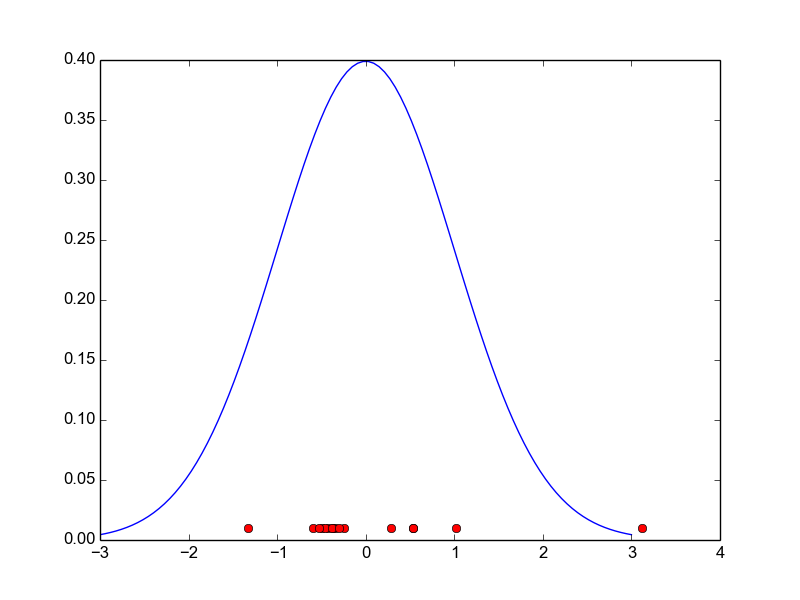
\includegraphics[width=5in]{imgs/iceland_dist.png}
 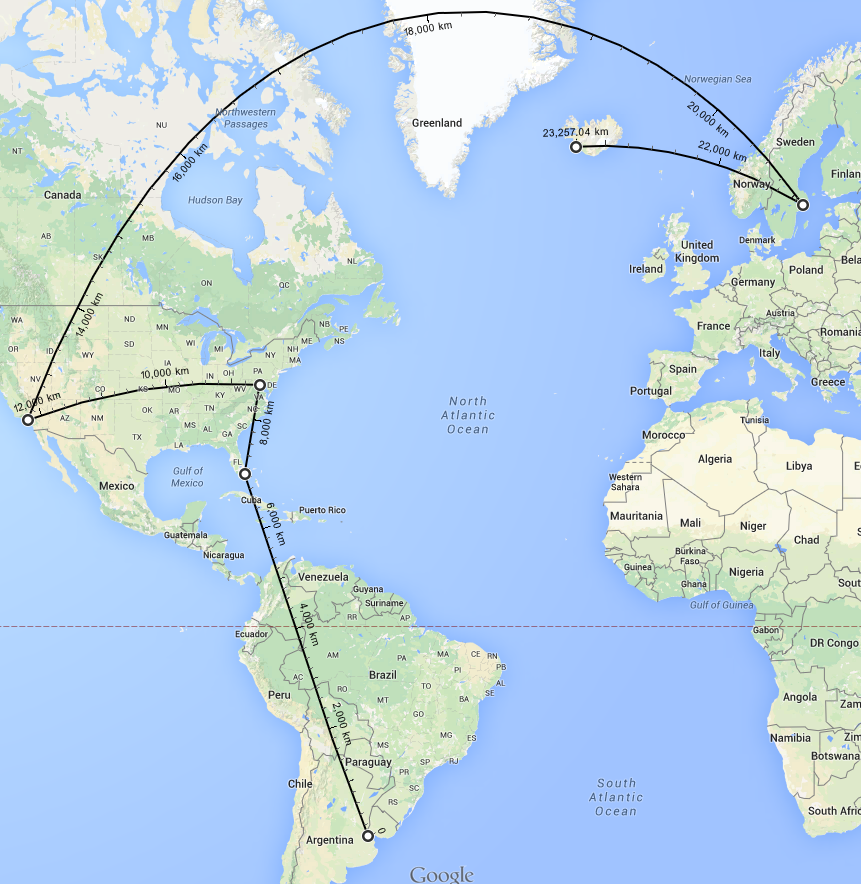
\includegraphics[width=5in]{imgs/maps/iceland2.png}


 Inicialmente los datos de geolocalización de esta ruta eran los que se muestran a continuación, que indicaban todos nodos en Miami hasta el salto a Suecia, pero esto no resultaba certero ya que entre los saltos en estados unidos había una variación muy alta (la correspondiente al salto hasta Los Angeles)

 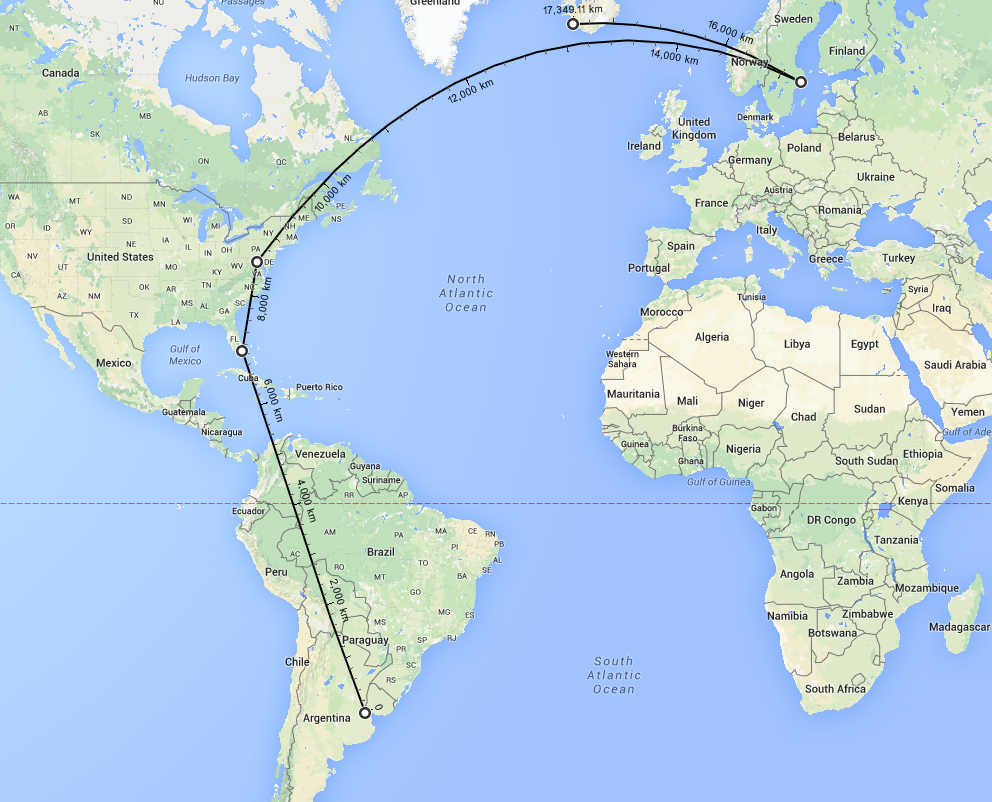
\includegraphics[width=5in]{imgs/maps/iceland.png}

\subsection{Perm, Rusia}

\begin{tabular}{|c@{\hspace{5ex}}c@{\hspace{5ex}}c@{\hspace{5ex}}c@{\hspace{5ex}}c|}
 \hline
 \rule{0pt}{1.2em}IP & ZRTT & AVG\_RTT & PAIS & CIUDAD\\[0.2em]
 \hline

\rule{0pt}{1.2em} 192.168.2.1  &  0.36 & 35.15 & (Private Address) & (Private Address) \\[0.2em]
\rule{0pt}{1.2em} 200.89.166.161  &  -0.30 & 45.49 & ARGENTINA & Buenos Aires \\[0.2em]
\rule{0pt}{1.2em} 200.89.165.130  &  -0.51 & 44.81 & ARGENTINA & Buenos Aires \\[0.2em]
\rule{0pt}{1.2em} 200.89.165.222  &  -0.46 & 46.45 & ARGENTINA & Buenos Aires \\[0.2em]
\rule{0pt}{1.2em} 208.178.244.213  &  -0.52 & 45.05 & ARGENTINA & Buenos Aires \\[0.2em]
\rule{0pt}{1.2em} 67.17.75.66  &  2.54 & 205.42 & UNITED STATES & Miami \\[0.2em]
\rule{0pt}{1.2em} 4.68.111.121  &  -1.06 & 175.47 & UNITED STATES & Miami \\[0.2em]
\rule{0pt}{1.2em} 4.69.158.245  &  1.89 & 301.85 & SWEDEN & Stockholm \\[0.2em]
\rule{0pt}{1.2em} 4.69.158.245  &  -0.42 & 305.45 & SWEDEN & Stockholm \\[0.2em]
\rule{0pt}{1.2em} 213.242.110.198  &  -0.26 & 317.85 & SWEDEN & Stockholm \\[0.2em]
\rule{0pt}{1.2em} 194.85.40.229  &  -0.29 & 328.49 & RUSSIAN FEDERATION & Saint Petersburg \\[0.2em]
\rule{0pt}{1.2em} 194.226.194.22  &  0.01 & 355.20 & RUSSIAN FEDERATION & Saint Petersburg \\[0.2em]
\rule{0pt}{1.2em} 212.192.80.57  &  -0.57 & 351.03 & RUSSIAN FEDERATION & Perm \\[0.2em]
\rule{0pt}{1.2em} 212.192.64.44  &  -0.37 & 357.50 & RUSSIAN FEDERATION & Perm \\[0.2em]
\hline
 \end{tabular}

 Nuevamente hace falta ``pasar por'' Miami para llegar a Europa, y una vez más el ZRTT es consistente con este salto.
 Inicialmente esta ruta fue complicada de analizar, ya que obteníamos un salto transatlántico sorprendentemente corto.
 Luego de corroborar mejor nuestras fuentes de geolocalización IP lo mismo cobró más coherencia observando que el salto transatlántico entre Estados Unidos y Suecia era lo que tenía el ZRTT alto.


 El throughput estimado para esta ruta fue de 3,923, nuevamente un valor comparativamente alto aunque no tanto como con el enlace con Islandia.

 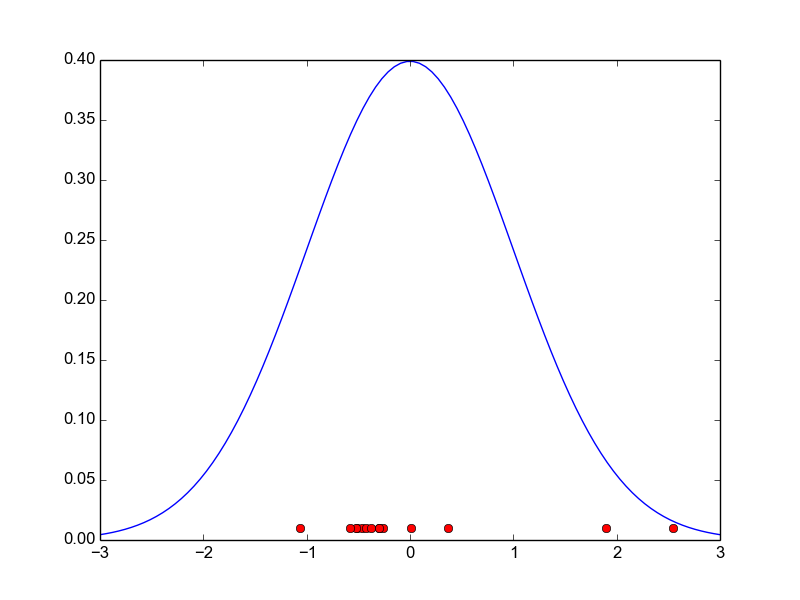
\includegraphics[width=5in]{imgs/perm_dist.png}
 \includegraphics[width=5in]{imgs/maps/perm.png}

\subsection{Pretoria, South Africa}

\begin{tabular}{|c@{\hspace{5ex}}c@{\hspace{5ex}}c@{\hspace{5ex}}c@{\hspace{5ex}}c|}
 \hline
 \rule{0pt}{1.2em}IP & ZRTT & AVG\_RTT & PAIS & CIUDAD\\[0.2em]
 \hline

\rule{0pt}{1.2em} 192.168.2.1  &  0.42 & 35.29 & (Private Address) & (Private Address) \\[0.2em]
\rule{0pt}{1.2em} 200.89.164.177  &  -0.20 & 45.07 & ARGENTINA & Buenos Aires \\[0.2em]
\rule{0pt}{1.2em} 200.89.165.130  &  -0.38 & 44.64 & ARGENTINA & Buenos Aires \\[0.2em]
\rule{0pt}{1.2em} 200.89.165.222  &  -0.36 & 45.49 & ARGENTINA & Buenos Aires \\[0.2em]
\rule{0pt}{1.2em} 208.178.195.205  &  -0.43 & 42.76 & ARGENTINA & Buenos Aires\\[0.2em]
\rule{0pt}{1.2em} 67.17.106.162  &  2.64 & 211.71 & UNITED STATES & Miami \\[0.2em]
\rule{0pt}{1.2em} 154.54.13.61  &  -1.14 & 168.90 & UNITED STATES & Atlanta \\[0.2em]
\rule{0pt}{1.2em} 154.54.24.233  &  -0.37 & 169.24 & UNITED STATES & Atlanta \\[0.2em]
\rule{0pt}{1.2em} 154.54.24.197  &  -0.13 & 183.11 & UNITED STATES & Atlanta \\[0.2em]
\rule{0pt}{1.2em} 154.54.31.110  &  -0.20 & 193.00 & UNITED STATES & Atlanta \\[0.2em]
\rule{0pt}{1.2em} 154.54.7.26  &  -0.28 & 198.41 & UNITED STATES & Chicago \\[0.2em]
\rule{0pt}{1.2em} 154.54.31.118  &  -0.39 & 197.44 & UNITED STATES & New York \\[0.2em]
\rule{0pt}{1.2em} 154.54.30.186  &  1.13 & 282.38 & UNITED KINGDOM & London \\[0.2em]
\rule{0pt}{1.2em} 130.117.50.201  &  -0.44 & 278.99 & ITALY & Milan \\[0.2em]
\rule{0pt}{1.2em} 154.54.38.190  &  -0.22 & 287.66 & UNITED KINGDOM & London \\[0.2em]
\rule{0pt}{1.2em} 149.14.80.210  &  -0.01 & 308.23  & UNITED KINGDOM & London \\[0.2em]
\rule{0pt}{1.2em} 196.32.209.50  &  -0.66 & 292.33 & SOUTH AFRICA & Cape Town \\[0.2em]
\rule{0pt}{1.2em} 196.32.209.117  &  3.08 & 485.75 & SOUTH AFRICA & Cape Town \\[0.2em]
\rule{0pt}{1.2em} 155.232.6.86  &  -0.63 & 471.57 & SOUTH AFRICA & Wynberg \\[0.2em]
\rule{0pt}{1.2em} 155.232.6.29  &  -0.07 & 488.65 & SOUTH AFRICA & Wynberg \\[0.2em]
\rule{0pt}{1.2em} 155.232.6.138  &  -0.66 & 472.79 & SOUTH AFRICA & Wynberg \\[0.2em]
\rule{0pt}{1.2em} 137.215.99.2  &  -0.17 & 484.43 & SOUTH AFRICA & Pretoria \\[0.2em]
\rule{0pt}{1.2em} 137.215.10.70  &  -0.45 & 480.05 & SOUTH AFRICA & Pretoria \\[0.2em]
\hline
 \end{tabular}

 Por lejos nuestra ruta más larga, lo primero que notamos es que a pesar de la relativa cercanía geográfica, para conectar Sudamérica con África hace falta pasar por continentes del norte (y una vez más por Miami, casi una constante de todas las rutas elegidas). Esta vez el salto trasatlántico sí tiene un ZRTT grande (más de un desvío standard) y el otro salto significativo es dentro de Cape Town, en Sudáfrica, cosa extraña.
 Creemos puede tener que ver con algún tipo error de geolocalización, aunque en varias bases de datos con fechas diferentes de actualización la localización resultaba consistente.
 La demora inducida en estos saltos pareciera muy grande para tratarse de demoras de encolamiento o situaciones similares en loops locales de Sudáfrica.

 Además, hemos re-analizado la diferencia entre los hosts 196.32.209.50 y 196.32.209.117 por separado, ya que ambos responden al ping, con herramientas adicionales (comando ping de Linux) como para verificar mejor esta situación puntualmente. Estos checkeos nos dieron resultados similares a los calculados por nuestra herramienta. Aproximadamente 175ms de diferencia.


 El throughput estimado para esta ruta fue de 3,030, el más bajo de las rutas usadas. Entendemos que tiene que ver con la gran distancia física que recorre la conexión trazada y su consiguiente RTT mayor a las demás rutas.

 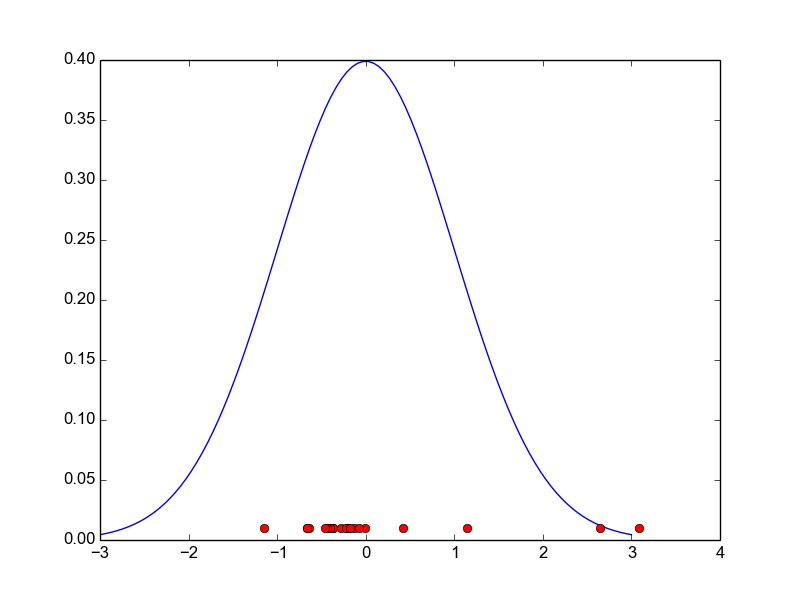
\includegraphics[width=5in]{imgs/pretoria_dist.png}
 \includegraphics[width=5in]{imgs/maps/pretoria.png}

\clearpage

\section{Conclusiones}
En el trabajo práctico trabajamos analizando las rutas que siguen los paquetes para llegar a distintos destinos de nuestro interés. Para lograr dicho objetivo, desarrollamos una herramienta que realiza un echo request al destino pero incrementando el valor TTL del paquete ICMP de a una unidad. De esta forma los distintos hosts que el paquete transita nos devuelven un \textit{Time Exceeded} como respuesta junto con su IP, haciendo posible, además de su identificación y un orden de los mismos, un calculo de RTT. Midiendo diferencias significativas en el valor de RTT logramos identificar los enlaces submarinos que conectan al mundo entre sí.

En el intento de medir hasta que host llega el paquete ICMP con determinado TTL o si llega a destino, nos encontramos con que algunos de los hosts no respondían nada. Esto resulta de la configuración de los mismos que por medidas de seguridad no permiten, o bien responder paquetes o bien filtran paquetes ICMP. Estos hosts no fueron incluidos en el analisis de las rutas y los RTT finales de cada Hop incluyen el tiempo que toma transitar por Hosts que no registran estos paquetes. Como conclusión a esto, hoy en día no se puede fiar del uso de los paquetes ICMP para realizar traceroutes dado que no todos los routers están configurados para tratar con ellos. Por esta razón, creemos que utilizar paquetes TCP sería de mayor precisión para obtener todos los hops de una ruta aunque habría que constatarlo experimentalmente.

Nos encontramos con resultados interesantes cuando analizamos los datos. Por ejemplo, cuando intentamos realizar la gelocalización de los distintos IPs. En ese caso, existen IPs que tienen un rango correspondiente a un país específico pero físicamente estan ubicados en otras regiones del mundo, lo que dificultó la ubicación de los mismos y la creación de los distintos mapas. Por otro lado, mediante la detección de cambios de ruta, pudimos observar que países como India tienen una alta redundancia en sus rutas (o un problema en su red), ya que se detectaron muchos cambios de rutas al realizar las repeticiones. Ademas, notamos que habian muchas universidades que no responden a un echo-request (por ejemplo la Universidad de Tokyo, Japón) por lo que se dificultó su selección.

Por otro lado, pudimos comprobar empíricamente la relación proporcional entre el RTT y la distancia geográfica de las rutas, y su relación inversa con el valor estimado por el throghput obtenido por la ecuación de Mathis, salvando algunas inconsistencias menores.

Descubrimos diferentes incosistencias entre las tablas de geolocalización IP, y tuvimos que tomar información de varias hasta encontrar datos consistentes con nuestros resultaods.

En un trabajo futuro, sería buena idea analizar las distintas rutas que puede tomar un paquete para llegar a destino, exponiendo los lugares por los que transita y los tiempos de cada uno de los caminos. También queda pendiente realizar este mismo análisis y otros utilizando paquetes TCP para mayor precisión.


\end{document}















